% 
% Annual CCN conference
% Sample LaTeX Two-Page Summary -- Proceedings Format
% based on the prior cognitive science style file
\documentclass[10pt,letterpaper]{article}

\usepackage{ccn}
\usepackage{subfig}
\usepackage{pslatex}
\usepackage{apacite}
\usepackage{graphicx}
\graphicspath{ {figures/} }
 


\title{Suboptimality in Human Sequential Planning}
 
\author{{\large \bf Zahy Bnaya (zahy.bnaya@nyu.edu)} \\
Center For Neural Science, New York University\\
  \AND {\large \bf Weiji Ma (weiji.ma@nyu.edu)} \\
Center For Neural Science, New York University\\
}

\begin{document}

\maketitle

\section{Abstract} {\bf


	Sequential planning is a difficult task that people generally do not solve optimally. Not much is known about how people are handing these tasks. 
	We use the game of rush-hour to study certain aspects of sub-optimally of human subjects. We collected data from 10 subjects and we show patterns in their solutions and that their response times are affected by distance to the goal. 

%The abstract should be identical to the text version submitted in the webform and should not exceed 1,500 characters, including spaces and any special characters. The       abstract should thus be relatively short. Aim for 150 words.
%Max length is 200 words. Arbitrarily long German words like "Donaudampfschiffartskapit\"an" are not encouraged.
%CCN has an interdisciplinary audience. Hence a good abstract should
%(a) give context about what the problem is and why it matters
%(b) give the contents and explain what was done and what was found
%(c) give a clear conclusion including what we learned and how it changes
%the way we think about the universe.
}

\begin{quote}
\small
\textbf{Keywords:} 
decision making; human behavior; planning; heuristic search
\end{quote}

\section{Planning in Fully Observable Deterministic Environments}

In sequential planning, the task is to find a strategy for achieving specific goal, based on descriptions of the initial state of the world, the desired goals and the set of possible actions. Planning tasks can be difficult even when the environment is deterministic and fully observable.
The common approach in Artificial Intelligence is to search the state space until such a strategy is found.

On simple cases, the optimal solution can be found using simple uninformed search such as Breadth-First-Search or Depth-First-Search. Tasks with larger state space require using heuristic search algorithms such as $A^*$~\cite{(Hart and Nillsen)} or $IDA^*$~\cite{(Korf)}. These algorithms  are still guaranteed to find the optimal solution under certain conditions.
However, humans are not optimal planners. This might be due to their limited memory or computational abilities, but the reasons and mechanisms behind human sub-optimality in planning are still largely unknown. Many search algorithms are designed for \emph{satisficing planning}, introducing many principled ways to deal with memory or computational limitations. Some algorithms perform partial search, such as online-search ~\cite{RTA*}or agent-centered search~\cite{Sven}. Others use hierarchical search~\cite{Dananau}. There are bounded suboptimal algorithms such as WA*~\cite{} algorithms and other algorithms that involve using inadmissible heuristic functions. These methods efficiently sacrifice optimality in favor of tractability of larger tasks, usually showing significant increase in solution capability without dramatically damaging the solution quality; some of these methods also have strict quality bounds. 

That might not be the case for humans.  It is not clear how much of the sub-optimality demonstrated by humans stems from efficient manipulation of their limited computational abilities such as the methods of AI.  One reason for this lack of understanding is the difficulty in modeling, estimating and testing such behavior. 

Our goal in this paper is to study how people behave sub-optimally when it comes to sequential planning in deterministic, single agent, fully observable tasks. 
We use the game of rush-hour (\url{www.thinkfun.com/play-online/rush-hour/}) as a testbed and provide preliminary results of our collected data.

\section{Experimental Results}

% TODO: reference
% TODO: Abstract
% TODO: Use facet.grid in fig:puzzle
% TODO: Add results of two other subjects
% TODO: Real results - real-dist
% TODO: real results - total expansions per instance 

\begin{figure}[ht]
\begin{center}
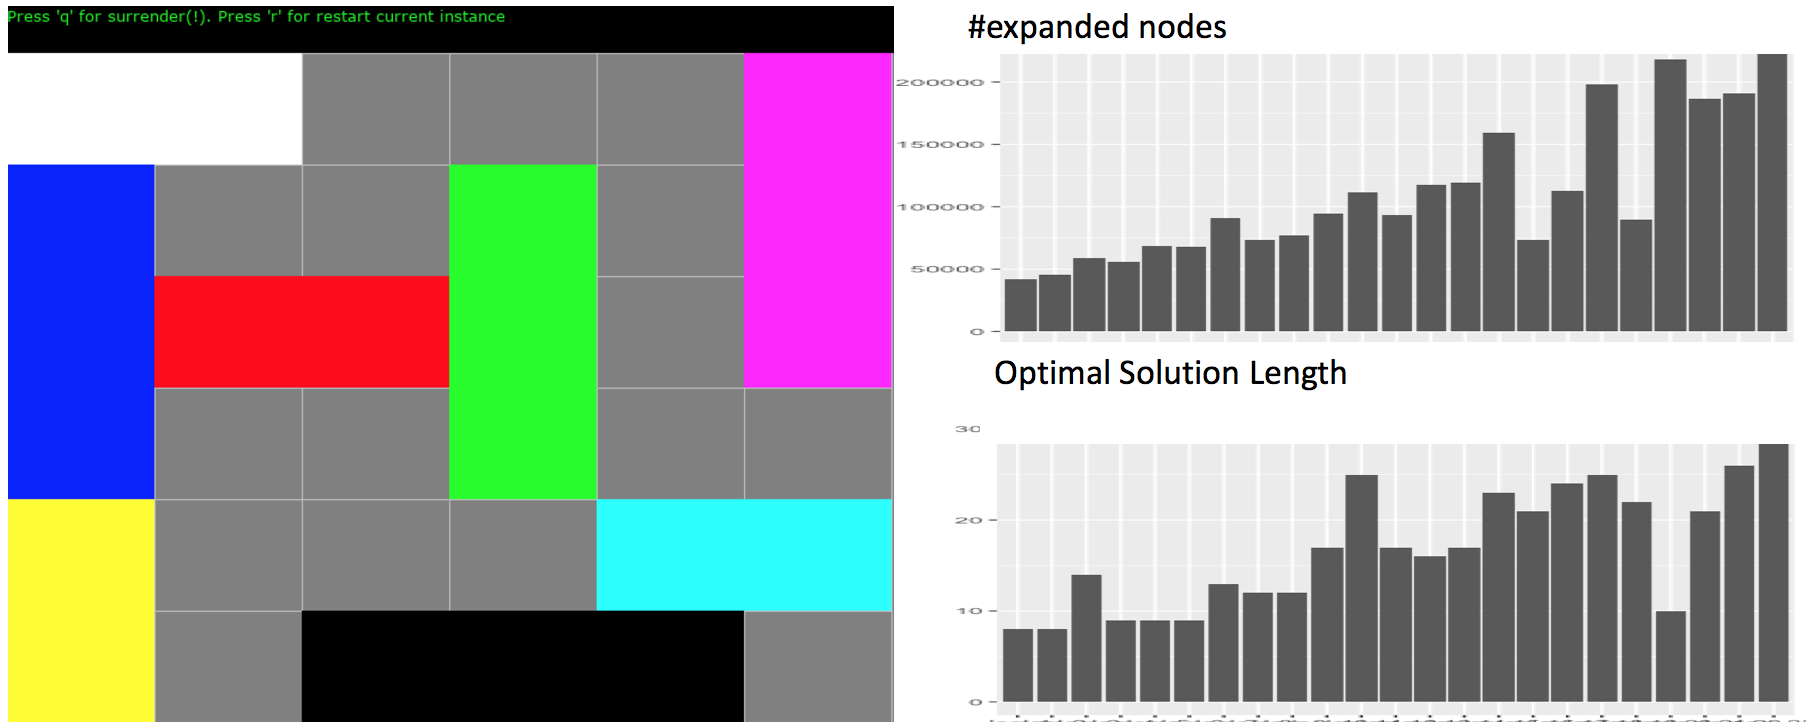
\includegraphics[width=0.5\textwidth]{puzzle}
\end{center}
\caption{(a) Example of rush-hour Puzzle. (b) number of expanded nodes by an optimal solver for every puzzle ordered by appearance (c) minimal solution length for every puzzle} 
\label{fig:puzzle}
\end{figure}

We asked 10 subjects to solve up to 40 rush-hour puzzles. Our subjects used a mouse and a keyboard to move cars on the screen. On all puzzles, the goal is to move the red car to the right edge of the screen. Figure~\ref{fig:puzzle}(a) shows an example puzzle.  We imposed a time limit of 30 minutes, after which the subject could complete the current puzzle.
Upon completion of a puzzle, the subjects automatically move to solve the next one. 
Subjects completed on average 13 puzzles, varying between 23 and 7 puzzles per subject. 
The order of puzzles was arbitrary chosen but with a tendency to increase in difficulty. Figure~\ref{fig:puzzle}(b) shows the  minimal number of actions required to solve the puzzle and Figure~\ref{fig:puzzle}(c) shows the number of expanded nodes needed for our optimal solver (using $A^*$ algorithm with simple admissible heuristics).  
Subjects are allowed to surrender and move to the next puzzle (by pressing the "s" key), or restart the current puzzle (by pressing the 'r' key) at any point of the experiment.

Figure~\ref{fig:p1}(a) shows the number of moves required for our subjects to solve each puzzle in relation to the optimal solution length. 
On average, people had to perform XXX\% more moves than the optimal solution. The first instances (up to 10 steps) were solved optimally by XX percents of our subjects. 
None of our subjects solved all puzzles optimally. In total there were XX optimal solutions out of YY solution paths that our subjects tried.

Figure~\ref{fig:p1}(b) shows the mean human solution length in relation to the optimal solution length.
People tended not to restart or surrender. Out of the 10 subjects, three surrendered and only two surrendered more than once. On average subjects surrendered after three trials. Six subjects chose to restart a puzzle. Eight out of our puzzles were solved without anyone surrendering or restarting it. Figure~\ref{fig:p7} shows the overall number of restarts/skips and surrenders.

\begin{figure}[!htb]
	\centering
	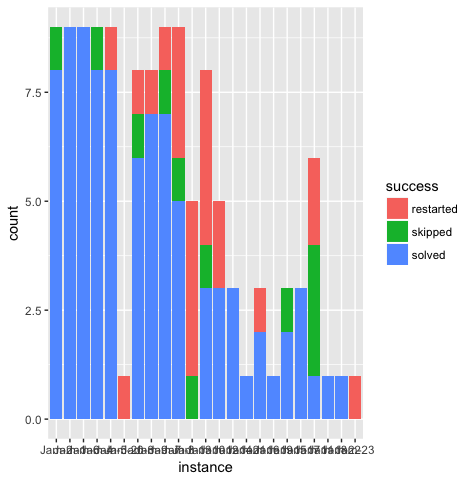
\includegraphics[width=0.5\linewidth]{p7}
	\caption{Restarts/Surrenders}
	\label{fig:p7}
\end{figure}


\begin{figure}
       \centering
       \subfloat[][]{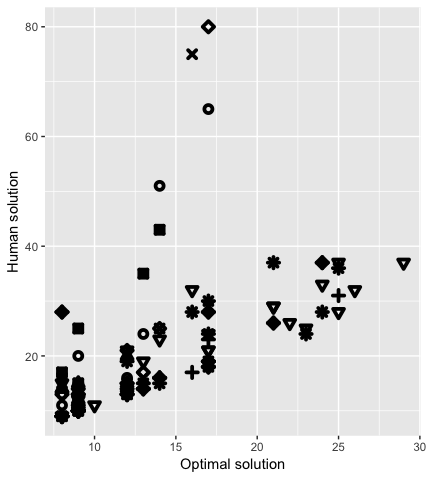
\includegraphics[width=0.5\linewidth]{p1}}
       \subfloat[][]{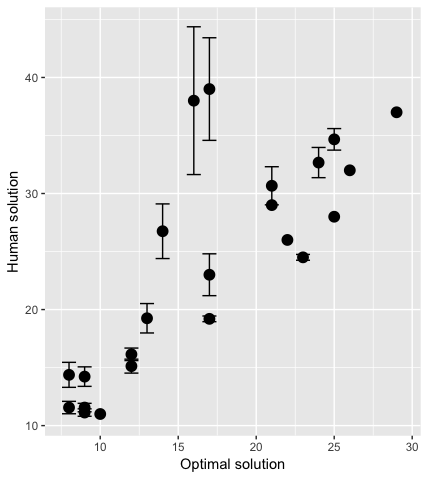
\includegraphics[width=0.5\linewidth]{p10_1}}
       \caption{(a) human solution vs. optimal solution. (b) mean human solution length in relation to the optimal solution}
       \label{fig:p1}
\end{figure}

During our experiment we also tracked the response times of our subjects for every move.  In general, our subjects spent more time on the first decision of each puzzle. Figure~\ref{fig:p3}(a) shows the scatter of response times in relation to the move number. Our subjects' response times were also affected by the distance from the goal (Figure~\ref{fig:p3}(b)). The overall distribution of response times is given in Figure~\ref{fig:p3}(c).

\begin{figure}
	\centering
	\subfloat[][]{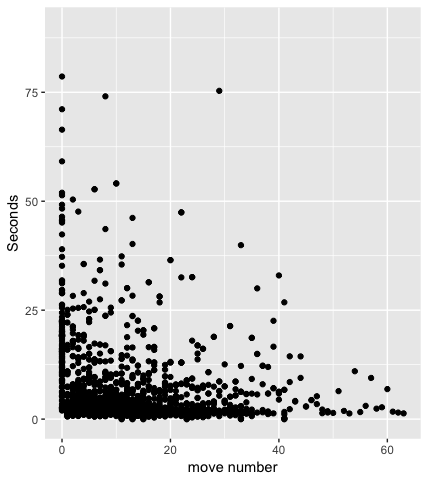
\includegraphics[width=0.34\linewidth]{p3_1}}
	\subfloat[][]{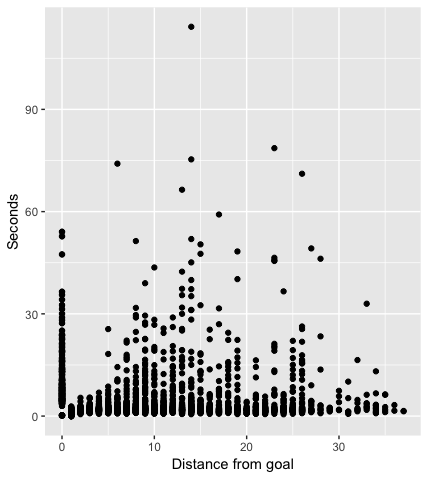
\includegraphics[width=0.34\linewidth]{p25}}
	\subfloat[][]{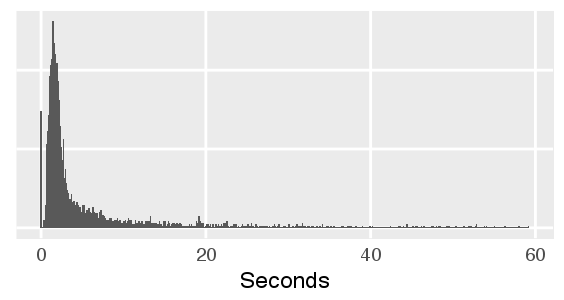
\includegraphics[width=0.34\linewidth]{p13}}
	\caption{(a) Response times vs move number (b) Response times vs. distance from goal (c) Response time distribution}
	\label{fig:p3}
\end{figure}

\begin{figure}[!htb]
	\centering
	\subfloat[][]{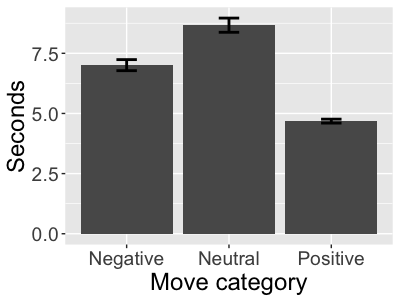
\includegraphics[width=0.5\linewidth]{p8_1}}
	\subfloat[][]{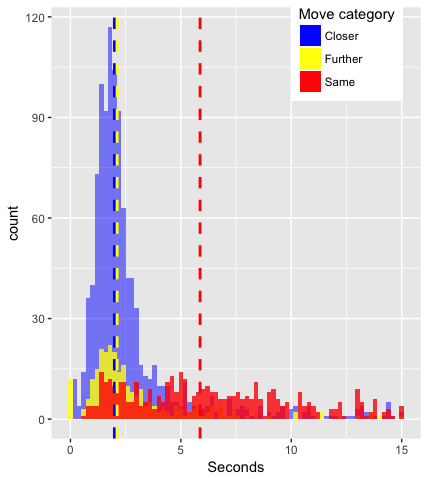
\includegraphics[width=0.5\linewidth]{p16}}
	\caption{(a) Response times per move category (b) Distribution of response times for move category}
	\label{fig:p8}
\end{figure}

\begin{figure}[!ht]
\begin{center}
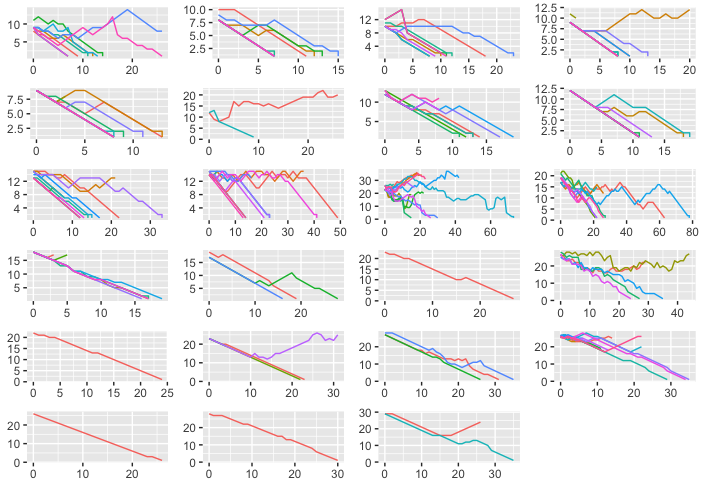
\includegraphics[width=0.4\textwidth]{p6}
\end{center}
\caption{Solution Progress} 
\label{fig:p6}
\end{figure}



\subsection{Solution progress}

We measure the progress of every solution attempt made by our subjects by calculating the minimal distance to the goal using an optimal solver, after every decision they made.  Figure~\ref{fig:p6} shows the progress of every solution attempt made by our subjects per puzzle. In general it seems that in many of our puzzles, subjects can recover from errors and move toward the goal. 
Another observation is that subjects tend to surrender or restart after they are getting far from the goal. This suggest that although the solution is not known, there is some awareness of the solution progress.
We category every move into positive, neutral or negative move, depending on whether it is getting the subject closer or farther to the goal, or keeping it the same. 
In total in our experiment, 1157 moves were positive, 291 negative and 509 neutral.

Figure~\ref{fig:p8} shows the mean number of moves made on each category across subjects.  Next, we look at the response times for move category.  
We also performed the Kruskal Wallis test to test whether the distribution of response time on each category is the same and found that not all three categories are the same.
It seems that our subjects spent more time on decisions that did not advance them in the solution.



%%The entire contribution of a short summary submission (including
%figures, references, and anything else) can be no longer than two
%pages. This short summary format is to be used for workshop and
%tutorial descriptions, symposia summaries, and publication-based
%presentation extended abstracts. Unlike submitted research papers,
%short summary submissions should \emph{not} begin with a separate
%abstract. Prior to the first section of the short summary, there
%should be the header ``{\bf Keywords:}'' followed by a list of
%descriptive keywords separated by semicolons, all in 9~point font, as
%shown above.
%
%The text of the paper should be formatted in two columns with an
%overall width of 7 inches (17.8 cm) and length of 9.25 inches (23.5
%cm), with 0.25 inches between the columns. Leave two line spaces
%between the last author listed and the text of the paper. The left
%margin should be 0.75 inches and the top margin should be 1 inch.
%\textbf{The right and bottom margins will depend on whether you use
%  U.S. letter or A4 paper, so you must be sure to measure the width of
%  the printed text.} Use 10~point Modern with 12~point vertical
%spacing, unless otherwise specified.
%
%The title should be in 14~point, bold, and centered. The title should
%be formatted with initial caps (the first letter of content words
%capitalized and the rest lower case). Each author's name should appear
%on a separate line, 11~point bold, and centered, with the author's
%email address in parentheses. Under each author's name list the
%author's affiliation and postal address in ordinary 10~point type.
%
%Indent the first line of each paragraph by 1/8~inch (except for the
%first paragraph of a new section). Do not add extra vertical space
%between paragraphs.
%
%
%\section{First Level Headings}
%
%First level headings should be in 12~point, initial caps, bold and
%centered. Leave one line space above the heading and 1/4~line space
%below the heading.
%
%
%\subsection{Second Level Headings}
%
%Second level headings should be 11~point, initial caps, bold, and
%flush left. Leave one line space above the heading and 1/4~line
%space below the heading.
%
%
%\subsubsection{Third Level Headings}
%
%Third level headings should be 10~point, initial caps, bold, and flush
%left. Leave one line space above the heading, but no space after the
%heading.
%
%
%\section{Formalities, Footnotes, and Floats}
%
%Use standard APA citation format. Citations within the text should
%include the author's last name and year. If the authors' names are
%included in the sentence, place only the year in parentheses, as in
%\citeA{NewellSimon1972a}, but otherwise place the entire reference in
%parentheses with the authors and year separated by a comma
%\cite{NewellSimon1972a}. List multiple references alphabetically and
%separate them by semicolons
%\cite{ChalnickBillman1988a,NewellSimon1972a}. Use the
%``et~al.'' construction only after listing all the authors to a
%publication in an earlier reference and for citations with four or
%more authors.
%
%
%\subsection{Footnotes}
%
%Indicate footnotes with a number\footnote{Sample of the first
%footnote.} in the text. Place the footnotes in 9~point type at the
%bottom of the column on which they appear. Precede the footnote block
%with a horizontal rule.\footnote{Sample of the second footnote.}
%
%
%\subsection{Tables}
%
%Number tables consecutively. Place the table number and title (in
%10~point) above the table with one line space above the caption and
%one line space below it, as in Table~\ref{sample-table}. You may float
%tables to the top or bottom of a column, or set wide tables across
%both columns.
%
%\begin{table}[!ht]
%\begin{center} 
%\caption{Sample table title.} 
%\label{sample-table} 
%\vskip 0.12in
%\begin{tabular}{ll} 
%\hline
%Error type    &  Example \\
%\hline
%Take smaller        &   63 - 44 = 21 \\
%Always borrow~~~~   &   96 - 42 = 34 \\
%0 - N = N           &   70 - 47 = 37 \\
%0 - N = 0           &   70 - 47 = 30 \\
%\hline
%\end{tabular} 
%\end{center} 
%\end{table}
%
%
%\subsection{Figures}
%
%Make sure that the artwork can be printed well (e.g. dark colors) and that 
%the figures make understanding the paper easy.
% Number figures sequentially, placing the figure
%number and caption, in 10~point, after the figure with one line space
%above the caption and one line space below it, as in
%Figure~\ref{sample-figure}. If necessary, leave extra white space at
%the bottom of the page to avoid splitting the figure and figure
%caption. You may float figures to the top or bottom of a column, or
%set wide figures across both columns.
%
%\begin{figure}[ht]
%\begin{center}
%\fbox{CCN figure}
%\end{center}
%\caption{This is a figure.} 
%\label{sample-figure}
%\end{figure}
%
%
%\section{Acknowledgments}
%
%Place acknowledgments (including funding information) in a section at
%the end of the paper.
%
%
%\section{References Instructions}
%
%Follow the APA Publication Manual for citation format, both within the
%text and in the reference list, with the following exceptions: (a) do
%not cite the page numbers of any book, including chapters in edited
%volumes; (b) use the same format for unpublished references as for
%published ones. Alphabetize references by the surnames of the authors,
%with single author entries preceding multiple author entries. Order
%references by the same authors by the year of publication, with the
%earliest first.
%
%Use a first level section heading, ``{\bf References}'', as shown
%below. Use a hanging indent style, with the first line of the
%reference flush against the left margin and subsequent lines indented
%by 1/8~inch. Below are example references for a conference paper, book
%chapter, journal article, dissertation, book, technical report, and
%edited volume, respectively.
%
%\nocite{ChalnickBillman1988a}
%\nocite{Feigenbaum1963a}
%\nocite{Hill1983a}
%\nocite{OhlssonLangley1985a}
%% \nocite{Lewis1978a}
%\nocite{Matlock2001}
%\nocite{NewellSimon1972a}
%\nocite{ShragerLangley1990a}
%

\bibliographystyle{apacite}

\setlength{\bibleftmargin}{.125in}
\setlength{\bibindent}{-\bibleftmargin}

\bibliography{sequential_planning}


\end{document}
